\section{Architecture} \label{architecture}

\subsection{Decentralized Governance Landscape} 
\label{decentralized_governance_landscape}
%\section{The Global Decentralized Governance Level}
%scope of this section
%There are two important questions related to governance: a) Who decides? and 
%b) 
%Who pays? Indeed, 
%this is true for any organization, or any system and it is also true for 
%blockchain systems. Decentralized governance on the other hand, essentially 
%means that the answer to these questions is: ``the community''. Cardano 
%aspires 
%to become a truly community-managed blockchain. A self-sustaining blockchain 
%system, where stakeholders can influence the future development of the network 
%and fund new development through a treasury system. However, decentralized 
%governance is a long journey. At the end of this journey -code-named the 
%Voltaire era- Cardano's future will be in the hands of the community! 
%
%What does it take to achieve decentralized governance? Can there even be a 
%``centrally governed decentralized system''? Isn't this an oxymoron? There are 
%many blockchain systems that claim that have achieved decentralized 
%governance, 
%but have they really? Imagine a blockchain system where the community 
%collectively decides what changes should be funded. However, when the change 
%is 
%implemented, then there is a trusted central authority who decides if this 
%implementation is appropriate to be deployed and when the changes will take 
%effect. Can we call this decentralized governance? It is important to 
%understand that governance does not have to do with just one decision. There 
%are a plethora of core decisions to be made in the whole lifecycle of a 
%change; 
%from the initial idea conception to the very end, where changes take effect 
%into the system. Decentralized governance requires to decentralize all 
%decision 
%points, or else it remains an utopia. 

In this section, we provide an overview of the overall Cardano 
decentralized governance landscape. We will identify the main components in 
this landscape and describe how these can be integrated into a global 
decentralized governance architecture.  We start by describing the main players 
in the governance game. We define what are the core decisions that have to be 
made and identify who is responsible to take each decision.  Then we move on to 
describe what are the main architectural components that provide the means for 
these decisions to be made collectively. To this end, we identify three 
components: a) the CIP process, b) the Treasury system and c) the Software 
updates system. The logical flow of a change through these three systems will 
essentially materialize decentralized governance in Cardano.

\paragraph{The main players}
These are the main players in Cardano decentralized governance:
\begin{itemize}
	\item \emph{The Cardano Community}. This is the community in the broader 
	sense. This means that there is no technical constraint in order to be part 
	of the Cardano community; for example the ownership of stake. Anyone could 
	participate. The community consists of Ada owners, Cardano enthusiasts, 
	Developers, stake pool operators, etc.
	\item \emph{The Stakeholders}. These are all the parties that own Ada.	
	\item \emph{The Stake Pool Operators (SPOs)}. SPOs are entities whose job 
	is to participate in the Proof-of-Stake consensus protocol, with the stake 
	that has been 
	\emph{delegated} to them by the 
	stakeholders. By doing this, SPOs earn rewards. They 
	cannot use the delegated stake to make transactions and thus 
	transfer the 
	money that they do not own.
	\item \emph{The Experts}. Experts are a still to-be-defined entity whose 
	purpose is to provide technical expertise to stakeholders, in order to help 
	them decide on governance issues, like the voting of a software update, the 
	funding of a proposal etc. Experts are rewarded for the services they 
	provide.	
\end{itemize}

\begin{figure}[h!] %[H]
	\centering
	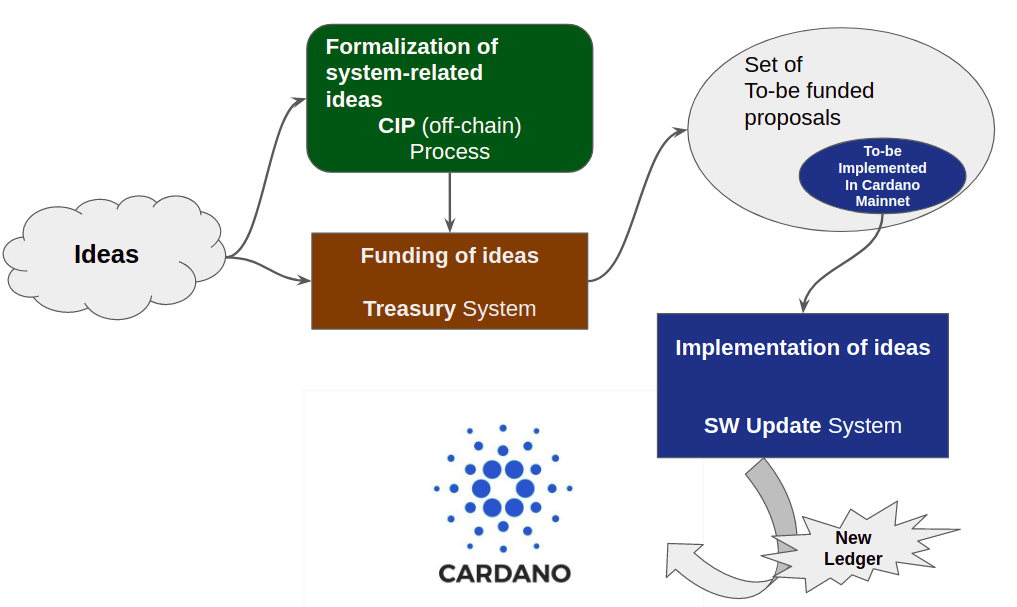
\includegraphics[width=0.8\columnwidth,
	keepaspectratio]{figures/cardano_dec_gov_components.png}
	\caption{The Cardano decentralized governance main components.}
	\label{fig:cardano_dec_gov_components}
\end{figure}

%what are the main components
%what is the main flow between these components
\paragraph{The main components}
In figure \ref{fig:cardano_dec_gov_components}, we identify three major 
components in the Cardano decentralized governance landscape.
\begin{itemize}
	\item \emph{The CIP Process}. \emph{CIP} stands for \emph{Cardano 
		Improvement Proposal} and it is a document. This document is the main 
	vehicle to formally describe and justify any \emph{idea} for improving the 
	Cardano system. It is similar in concept to BIPs (Bitcoin Improvement 
	Proposals)  and EIPs (Ethereum Improvement Proposals). The Cardano 
	Improvement process is intent on enabling a public discussion place for 
	``Cardano Improvement Proposals'' as Process, Standard or Informational 
	proposals, in a source-controlled, Foundation-managed, GitHub 
	repository.The aim is to have an open-sourced collection of CIPs available 
	and proposed for the community, enabling different flavors of 
	implementation and a varied ecosystem, maybe at first mostly curated by 
	IOHK/Emurgo/Cardano Foundation via a group of CIP Editors, but eventually 
	community-maintained. Getting an idea formalized in the repository provides 
	the foundation for solid conversation and public inquiry. From an 
	architectural perspective, please note that the CIP Process is an 
	\emph{off-chain} process.
	
	\item \emph{The Treasury System}. The Treasury system is the means by 
	which proposals and ideas can be funded in a collective, community-based 
	manner. Funds in this global, community-owned pot, are raised via taxation, 
	donations or other methods and are offered for the funding of new projects 
	through the process of \emph{funding ballots}. It is a fully-fledged 
	decentralized 
	governance system that utilizes advanced voting protocols, liquid democracy 
	models and advanced cryptography to ensure the secure and decentralized 
	operation of the Treasury. A good description of the research-related 
	issues regarding a Treasury system can be found in 
	\cite{treasury}. The Cardano Treasury system can 
	fund \emph{any} idea that improves the Cardano ecosystem and not 
	necessarily only system-related ideas; for example to launch a new 
	marketing campaign, or create educational material for the Cardano 
	community and so on. In fact, the system-related ideas, 
	i.e., the ones that will eventually become a \emph{software update} 
	proposal, are only a subset of the total set of the to-be funded proposals. 
	This is depicted in figure \ref{fig:cardano_dec_gov_components}.
	
	\item \emph{The Update system}. Finally, the Update system is the means for 
	implementing and applying to the Cardano blockchain all system-related 
	ideas. It is responsible for taking a software update through out all the 
	steps in its lifecycle, from ideation to implementation and finally the 
	activation of changes on the blockchain and do that in a secure but also 
	\emph{decentralized} manner.
	Of course, the Cardano update system is the main goal of this 
	PRIViLEDGE use case.
\end{itemize}
The basic flow depicted in figure \ref{fig:cardano_dec_gov_components}, shows 
that system-related ideas going through a formalization process, in the form of 
a CIP document. Non system-related ideas do not need this step. Some ideas 
might 
end up in the Treasury system 
requesting for funding and some others might not require funding at all (e.g., 
parameters value change). Finally, the subset of the proposals that correspond 
to software updates, will go through the SW 
Update system to enable the implementation of the initial idea and the 
activation of the changes on the blockchain system.

\begin{table}[h!]
	\centering
	\begin{tabular}{|| p{6cm} | c | c ||} 
		\hline
		Decision & Who & Means\\ [0.5ex] 
		\hline\hline
		What proposal should be funded? & Stakeholders & Treasury system  \\ 
		\hline
		What Cardano (system-related) improvement proposal (CIP) should move 
		forward? & Community & CIP off-chain Process  \\
		\hline
		What Design (SIP) should be approved for implementation? & Experts & SW 
		Updates System  \\
		\hline
		What Implementation of a design should be approved for deployment & 
		Experts & SW Updates System  \\
		\hline
		When should we activate the deployed changes (synchronization)? & 
		Stakepool Operators & SW Updates System  \\ [1ex] 
		\hline
	\end{tabular}
	\caption{Main decision of the decentralized governance circle.}
	\label{table:main_decisions}
\end{table}

%what are the main decisions?
We have seen that decentralized governance is all about community-driven 
decision making. Moreover, the components that we have described provide the 
means by which decisions can be made collectively; but what are the core 
decisions? In table \ref{table:main_decisions}, we list the main decisions of 
the decentralized governance circle. Also in this table, we propose which 
player 
should make the corresponding decision (''Who'' column) and via 
which component this decision process will take place (''Means'' column).

In the lifecycle of a software update, we identify three core decisions that 
are 
recorded in table \ref{table:main_decisions}. The first decision has to do with 
the approval of the \emph{design} of the update proposal. This design is 
formalized and submitted for review and approval via a technical document 
called \emph{System Improvement Proposal (SIP)}. The next important decision 
has to do with the approval of the implementation of the update proposal. 
Finally, for all approved implementations there is a final decision of when to 
activate the corresponding changes. This is critical because, if the parties in 
the Cardano network activate without appropriate \emph{synchronization}, then 
there is a risk for a chain split and for activating a new consensus protocol 
in which the security assumptions do not hold.

\begin{figure}[h!] %[H]
	\centering
	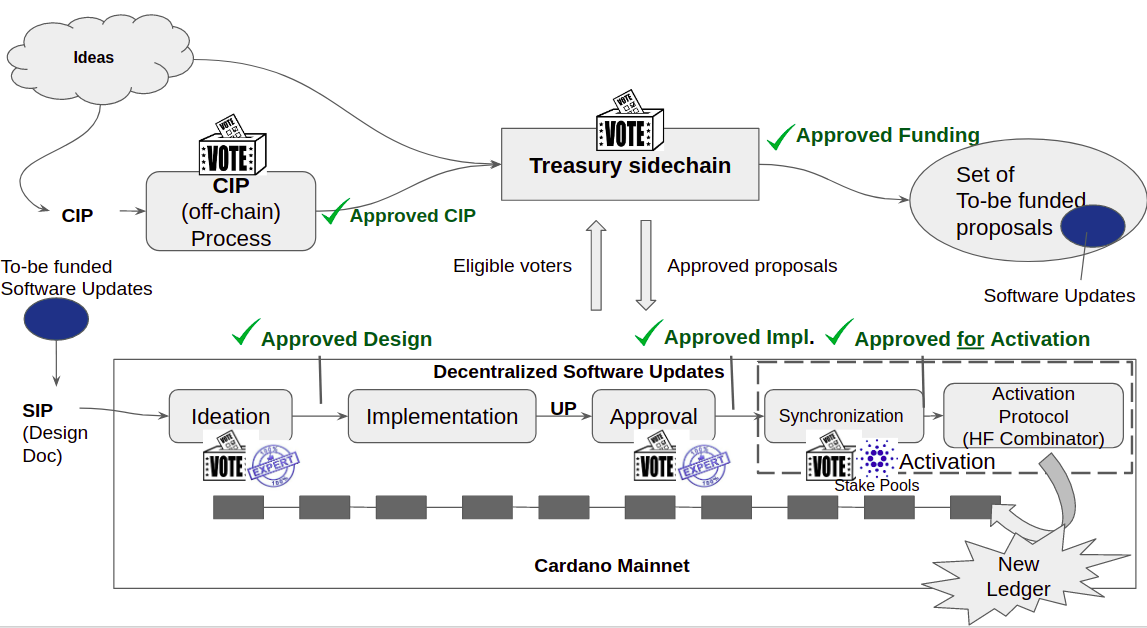
\includegraphics[width=0.8\columnwidth,
	keepaspectratio]{figures/cardano_dec_gov_landscape.png}
	\caption{The Cardano decentralized governance global architecture.}
	\label{fig:cardano_global_architecture}
\end{figure}

%global architecture
In figure \ref{fig:cardano_global_architecture}, we can see the Cardano 
decentralized global architecture. Observe that the aforementioned three main 
components of the decentralized governance landscape are depicted. In 
particular, the software updates system appears integrated with the Cardano 
main-chain and is depicted as a flow of the core phases in the lifecycle of a 
software update, namely: Ideation, Implementation, Approval and Activation. In 
contrast, the Treasury system runs as a sidechain \cite{sidechain}. This is a 
conscious architectural decision, which we explain next.

The update system enables changes on the main-chain, so it is very important 
that it is secure, because if the chain gets compromised or the protocol fails 
people can lose their money. So the chain upon which the update system runs 
must be \emph{at least} as secure as the main Cardano chain. This requirement 
calls for a tight integration between the update system and the Cardano node 
software, as we will show in section \ref{integration_with_cardano}. For 
example, 
the triggering for the activation of a change that comes from the update system 
is integrated within the ledger layer of the Cardano node (see section 
\ref{integration_with_cardano}). 

The high-stake nature of software updates mandates that on-chain decisions 
about them should be made on a chain that is at least as secure as the chain on 
which the changes will be applied . If we had followed a sidechain approach for 
the 
update system, then that would mean that the sidechain should be as secure as 
the main chain on which the changes will take effect. Moreover, we would have 
to utilize more advanced cryptography 
\cite{sidechain}, in order to provide strong evidence that indeed the 
changes should be activated on the main-chain. All these along with the 
requirement for a 
robust, simple-to-implement, fast-and-scalable and also transparent and 
auditable update mechanism has lead us to the decision to implement the update 
mechanism on the Cardano main-chain. In contrast, the Cardano Treasury system, 
which is implemented as a sidechain, deals with lower-stake decisions (the 
funding of projects) compared to software updates. Also, it has built advanced 
voting protocols and utilizes advance cryptography to ensure 
the privacy of the voters (something that is not required for the update system 
due to the transparency requirement and also because votes for 
updates must be open, in order for the experts to be accountable for their 
vote). By implementing the Treasury system as a sidechain, 
we eliminate the need to implement complex cryptographic algorithms on the 
Cardano chain and gives the ability to the Treasury team to experiment with 
different voting protocols and governance models, without the need to trigger 
hard forks on the Cardano chain.

In figure \ref{fig:cardano_global_architecture}, we can also see the main 
decision points in the governance cycle depicted as check-marks. We see and 
initial idea to take the form of a CIP and go through the off-chain CIP 
process. Then, once it is approved it is submitted to the Treasury system for 
requesting funding. The Treasury sidechain gets from the main-chain the list of 
eligible voters and a ballot is executed. If the funding gets approved, then 
the sidechain must interact with the main-chain in order to send the ballot 
result (in a secure undisputed way\footnote{The exact protocol for the 
	interaction of the Treasury sidechain with the Cardano main-chain is out of 
	the 
	scope of this document and thus omitted.}) and release the funds. Next, the 
approved 
proposal must be submitted on 
the main-chain as a SIP and the update protocol starts. During the Ideation 
phase a voting round will run, in order to approve the submitted SIP. In this 
voting process, experts will vote through a delegation process in place. 
Approved SIPs proceed in the implementation phase, the end-result of which is 
to submit the implementation for approval. This is the Approval phase of the 
update protocol where another voting round with the experts takes place, in 
order to review and approve the submitted implementation. The implementations 
that are approved move on to the Endorsement phase where parties (Stake Pool 
Operators) download and upgrade their software and signal their readiness for 
activating the changes. Once, the required \emph{adoption threshold} of 
endorsements has been reached, the update mechanism gives a green light to the 
activation protocol to run. This protocol will take care of transitioning to 
the new consensus protocol in a secure manner. This is 
implemented by a component called \emph{hard fork combinator}, which is shown 
in the figure and will be also discussed in the next section.

\subsection{Integration with Cardano Node} \label{integration_with_cardano}
%\section{The Intra-Node Level}\label{sec:intra-node-level}
The \emph{Cardano node} is the software that must be run by anyone who wants to 
be part of the the Cardano blockchain network. In particular, it is the 
software necessary in order to participate in the 
Ouroboros consensus protocol \cite{C:KRDO17}. In this section, we will take a 
closer look into the Cardano node internals and see where the update 
system fits within the Cardano node architecture. 

\begin{figure}[h!] %[H]
	\centering
	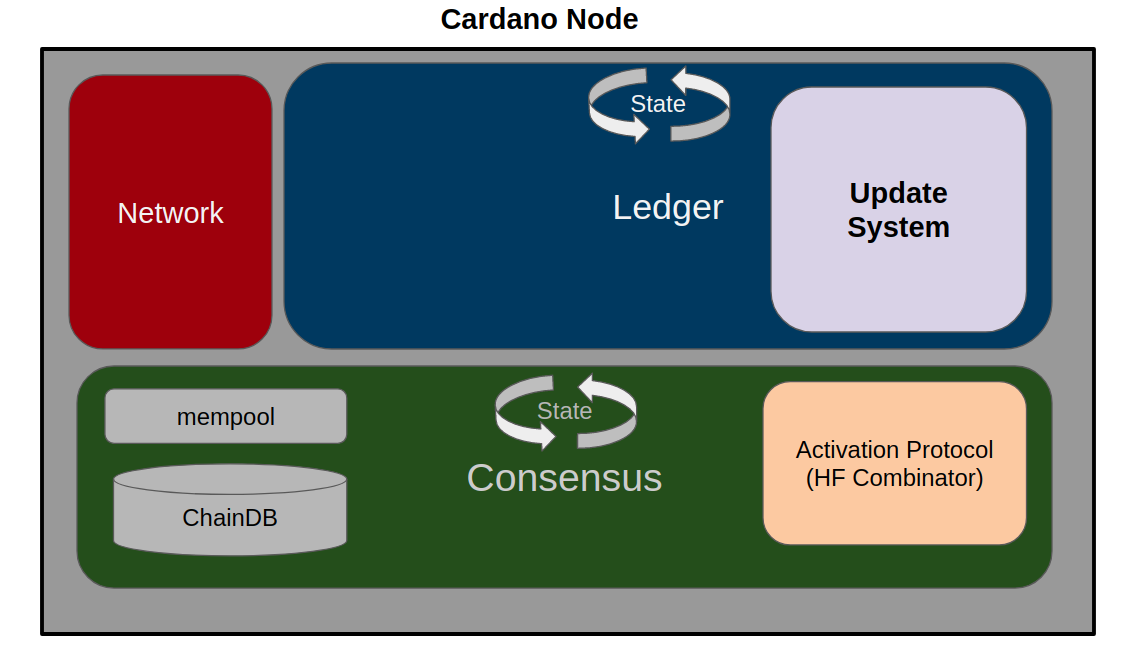
\includegraphics[width=0.8\columnwidth,
	keepaspectratio]{figures/cardano_node.png}
	\caption{The Cardano node architecture.}
	\label{fig:cardano_node}
\end{figure}

In figure \ref{fig:cardano_node}, we provide a very high level view of the 
Cardano node architecture. At its core, the Cardano node consists of three main 
components:
\begin{itemize}
	\item the consensus layer,
	\item the ledger layer and
	\item the network layer.
\end{itemize}
%describe consensus
The consensus layer is the heart of the node. It is where the Ouroboros 
consensus protocol \cite{C:KRDO17} is implemented. In this layer, the notion of 
the \emph{blockchain} is materialized. The consensus layer is 
responsible for deciding on and maintaining the \emph{chain of blocks} that 
will be the \emph{single version of the truth}. Based on this truth, the ledger 
layer 
will build the notion of a \emph{transaction ledger}. The primary job of the 
consensus layer is to ''listen'' for blocks from the network, or to create new 
blocks with transactions drawn from the \emph{mempool} and maintain the 
blockchain by faithfully following the directives of the consensus protocol. It 
implements all the logic how to handle forks and apply the \emph{chain 
	selection 
	rules}, so 
that there will always be a single chain of blocks exposed to the other 
components. The actual blockchain data are stored in a database called ChainDB. 
Also, we must note that this layer maintains its own specialized state, which 
updates with every operation taking place at the blockchain level.
Finally, it is important to stress that the consensus layer knows 
\emph{nothing} about the 
\emph{contents} of the blocks. This is the responsibility of the ledger layer.

%describe ledger
The ledger layer knows how to validate the contents of a block (including the 
block 
header). For this reason, the ledger layer is the ultimate authority within the 
node to decide if a block header, or a block is valid. Upon rejection 
of 
a block the consensus layer immediately discards the invalid 
block and blacklists the peer who transmitted it. Therefore, the ledger layer 
is where all the \emph{validation rules} are implemented. Moreover, since the 
ledger layer can interpret the contents of the blocks, i.e., the transactions, 
it is the place where the transaction logic is implemented. So the ledger layer 
knows what is a transaction that moves value from one party to another and 
maintains the \emph{ledger state} appropriately to correspond to the actual 
transfer of value. 

%describe network
Finally, the network layer is a specialized layer that tries to fulfill the 
network needs of the consensus layer. Naturally, the node has extensive needs 
of network communication, since it is a system that communicates directly with 
both upstream and downstream peers (i.e., other nodes), but also with clients 
like the wallet or the cli. Upstream peers are the nodes from which the 
node receives data (transactions or blocks) and downstream peers are the nodes 
to which a node sends data. Although in practice, in some cases, the 
distinction between the network and consensus layer is not so clear, at the 
level of detail we are discussing, it is sufficient to think the network layer 
as the main network services provider of the consensus layer.

%mention isolation principle
At this point, it is important to point out one significant design principle 
that has been followed in the Cardano node architecture, namely the
\emph{isolation principle}. Essentially, this means that the consensus layer 
knows nothing about transactions and their validity rules and similarly the 
ledger layer knows nothing about the actual blockchain with all its
forks and rollbacks taking place at the consensus protocol level. The consensus 
layer exposes to the ledger layer just a \emph{single} history of transactions, 
nicely grouped into blocks. Among the many features of this isolation principle 
a very important one is that one can thoroughly test each layer separately. 
Moreover, one can move to a new version of ledger rules without affecting the 
other layers.  

%describe update system as part of the ledger
In figure \ref{fig:cardano_node}, we can see the update system as a component 
\emph{within} the ledger layer. Indeed, just like the ledger layer is the 
ultimate authority for validating the contents of a block, i.e., transactions, 
similarly the update system is the sole responsible for interpreting the 
special content of a transaction that is called the \emph{update payload}. In 
our software updates solution, update events are transmitted via the payload 
(i.e., metadata) of individual transactions. This is a design choice that 
enables: a) the open participation in the update protocol by anyone (i.e., 
stake owner) who can submit a common transaction and b) the enforcement of a 
\emph{fee} with every update event transmitted, which is a protection against 
denial of service attacks. Therefore, the ledger layer knows nothing about the 
update payload and needs the update system sub-component to validate this 
payload and act upon it by updating appropriately the ledger state.

%describe the HF combinator
The last component of figure \ref{fig:cardano_node} that we need to describe is 
the \emph{hard fork combinator} (HFC). This is a specialized 
component residing in the consensus layer. Its sole purpose is to execute 
securely the transition from the current consensus protocol to the upgraded 
consensus protocol triggered by a software update. The HF combinator implements 
a secure activation protocol such as the ones that we have proposed recently 
\cite{secure_activation}. Please note that the HF combinator does not know when 
to initiate the transition, i.e., when the security conditions hold for such an 
endeavor; it only knows how to execute the transition. The trigger for 
initiating the activation must come from the component that implements the 
\emph{update logic} and knows when it is the right time to activate; this is of 
course the update system within the ledger layer.

\begin{figure}[h!] %[H]
	\centering
	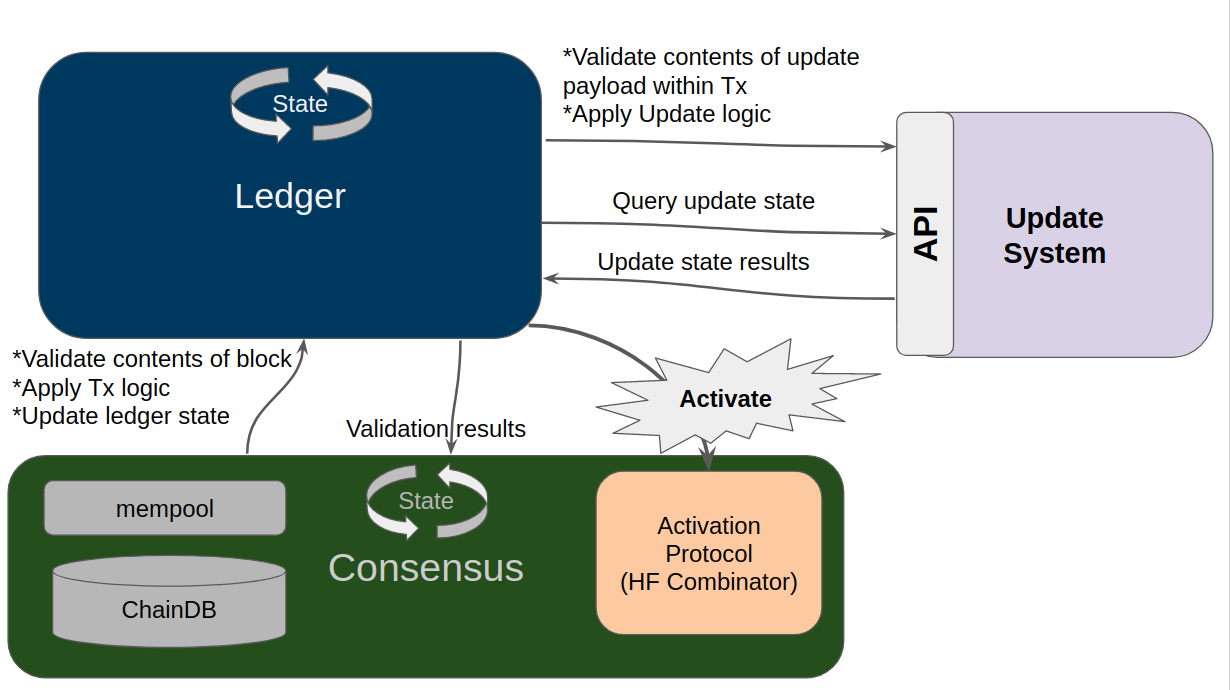
\includegraphics[width=0.8\columnwidth,
	keepaspectratio]{figures/cardano_node_integration.png}
	\caption{The integration of the update system in the Cardano node.}
	\label{fig:cardano_node_integation}
\end{figure}

%describe the integration of the update system with the other components
Finally, in figure \ref{fig:cardano_node_integation}, we depict how the 
integration of the update system within the node architecture is actually 
implemented. Starting at the bottom of the picture, we can see the consensus 
layer handing over to the ledger layer the contents of a block (i.e., 
transactions) to be validated and wait to get back the validation results. The 
ledger layer is responsible for validating each transaction except for one 
particular case: the update payload. Therefore, in the figure, we can see the 
ledger layer interacting with the update system through a well-defined 
\emph{API} that the latter exposes to the outside world. Basically, 
through this API, the ledger layer can hand over to the update system a 
specific update payload. The update system validates this update-specific 
payload (e.g., a proposal submission, a vote for a proposal, an endorsement of 
a proposal etc.) and applies the appropriate \emph{update logic}. Furthermore, 
with each and every update event the update system maintains its own update 
state and offers a state query interface through the exposed API. The ledger 
constantly queries the update state and in turn updates the ledger state. 
Finally, the ledger layer ''asks'' the update system when it is the right time 
to activate a change and only when the update system gives the green light, 
then the ledger layer triggers the HF combinator to activate the changes.


\subsection{Prototype Architecture} \label{software_architecture}
%\section{The Update System Level}
In this section we describe the 3rd level of detail of our proposed 
architecture that of the update system per se. For the convenience of the 
reader, we start with a short overview of the decentralized software update 
lifecycle, the phases of which, the update system essentially implements.

\ignore{
\subsubsection{An Overview of the Decentralized Software Update
	Lifecycle}\label{sec:su_lifecycle}
In order to understand the logic that the update system implements, we need to 
closely follow a software
update through out its whole life-cycle; from the very first phase, where it is
born as an idea, to the last phase, where the changes are activated on the
blockchain. In deliverable \emph{D4.1 Report on Architecture of Secure Ledger
	Systems}, we have provided a detailed description of all the steps in the 
said
lifecycle. In this section, we only provide a brief overview (see figure
\ref{fig:su_lifecycle}), in order to set the context for the reader's
convenience.

\begin{figure}[h!] %[H]
	\centering
	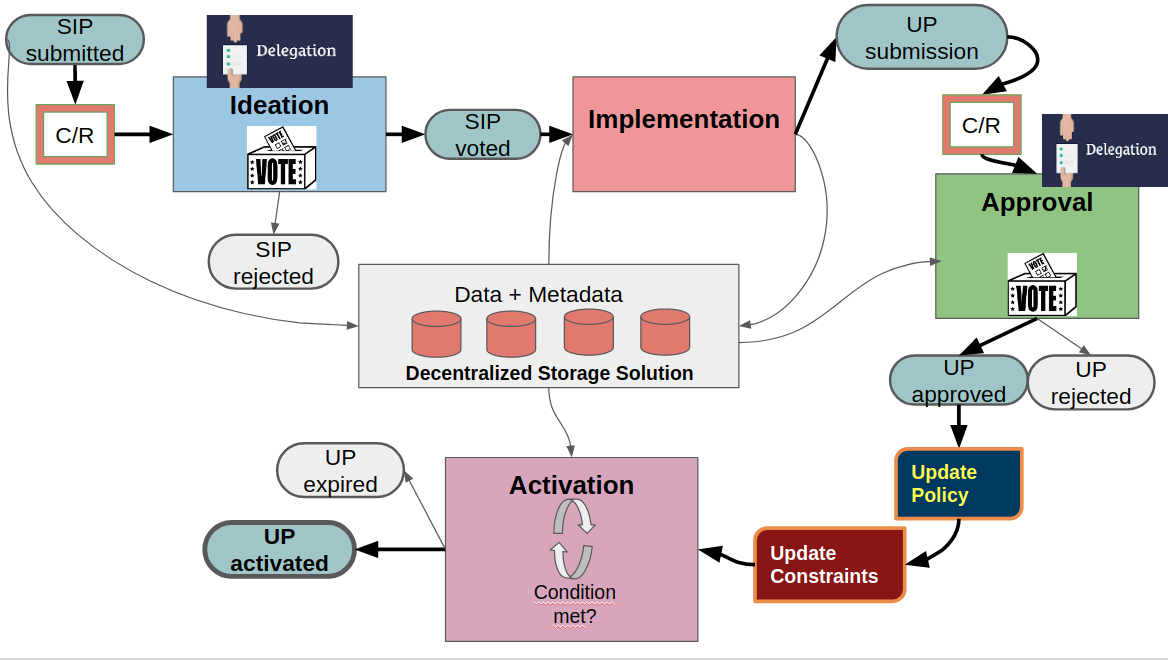
\includegraphics[width=0.8\columnwidth,
	keepaspectratio]{figures/software_update_lifecycle.png}
	\caption{The Decentralized Software Update Lifecycle.}
	\label{fig:su_lifecycle}
\end{figure}

A software update starts its life as a \emph{System Improvement Proposal
	(SIP)}, which is submitted to the blockchain. This submission takes place 
with
a fee-based transaction, which carries the proposal in its metadata
(\emph{transaction payload}). A SIP is a structured document
describing an update proposal. This submission goes through a typical
\emph{commit-reveal scheme}, in order to ensure the rightful authorship of the
proposal. Once the SIP is revealed, a voting period starts for this SIP; the
software update has entered the \emph{Ideation phase}. The duration of the
voting period is metadata-driven, i.e., defined in the SIP
metadata\footnote{There is an upper limit for the voting period duration in the
	implementation, to prevent DoS attacks.}.

The purpose of the Ideation phase is to help the community decide which SIP
will move forward to the next phase. Votes are also fee-based transactions with
a special payload. Anyone who owns enough stake to make a transaction can
potentially vote. Votes count proportionally to the owned stake. Votes are
accepted only within the voting period and multiple proposals can compete in
parallel. The outcome (verdict) of the voting process for a specific proposal
might be: a) \emph{Accepted}, when stake in favor is above a threshold, b)
\emph{Rejected}, when stake against is above a threshold, c) \emph{No Quorum},
when stake abstaining is above a threshold; this outcome leads to revoting, d)
\emph{No Majority}, when non of the previous three results occur, which also
leads to revoting and e) \emph{Expired}, when after the maximum number of
revoting periods has been reached and still the proposal was neither been
accepted or rejected. Finally, note that for the voting, we allow delegation of
a stakeholder's voting right to an \emph{expert}. For the scope of our
prototype implementation we have assumed delegation as an out-of-band solution
and provided direct voting power to stakeholders. This is basically for two
reasons: a) to reduce risks in the prototype implementation (especially of the
Cardano integration part) and b) to defer introducing delegation to experts
until a proper game-theoretic analysis of the expert's incentives has been
completed.

The \emph{Implementation} phase is an off-chain process, where an approved SIP
is implemented. It ends with the submission of the implementation, which we
formally call \emph{Update Proposal (UP)}\footnote{We will use the terms
	\emph{UP} and \emph{Implementation} interchangeably}, to the blockchain. 
Once
this UP is
revealed, the we have entered the \emph{Approval} phase. This is the phase
where the community is called to approve a submitted implementation. The voting
process and the technical details are similar to the Ideation
phase. Once the
UP is approved it enters the \emph{Activation} phase depicted in figure
\ref{fig:activation_phase}.

\begin{figure}[h!] %[H]
	\centering
	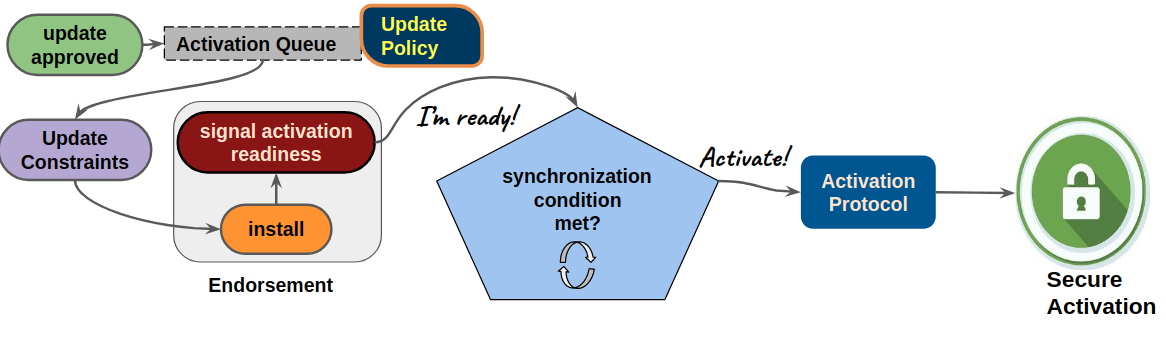
\includegraphics[width=0.8\columnwidth,
	keepaspectratio]{figures/activation_phase.png}
	\caption{The Activation Phase.}
	\label{fig:activation_phase}
\end{figure}

An approved update proposal enters the activation phase and is placed in the
\emph{activation queue}. At this point, the
\emph{update constraints} of the proposal will be evaluated. A proposal
satisfies the update constraints when:
\begin{itemize}
	\item is approved,
	\item meets its dependencies,
	\item does not conflict with the current version,
	\item has the highest priority among competing proposals
\end{itemize}

If a proposal satisfies its update constraints it enters the \emph{Endorsement
	Period}. This is the period where the \emph{block issuers} download and
install the update and \emph{declare} upgrade readiness. Note that only a
\emph{single} proposal can be endorsed at a time. The endorsement period lasts
$N$ number of \emph{epochs}, which is a metadata-defined parameter, called the
\emph{safety lag}; the safety lag corresponds to the sufficient deployment time
window required for the specific update proposal. Once the endorsements reach a
specific stake threshold, called the \emph{adoption threshold}, the activation
gives the green light to the \emph{activation protocol} to run. The activation
protocol ensures the secure activation, i.e., the secure transfer from the old
ledger to the upgraded ledger, based on our formal definition of activation
security and corresponding security proofs \cite{secure_activation}. In a
nutshell, \emph{secure activation} means, the secure transition from the old
ledger (L1) to the new ledger (L2) in a way where:
\begin{itemize}
	\item L2 enjoys liveness
	\item L2 enjoys consistency
	\item L2 has L1 as a prefix
\end{itemize}

Finally, note that the
all the metadata-defined information about an update proposal, such as the
deployment window length, the proposal's priority, the version dependencies
etc., form the proposal's \emph{update policy} to be followed by the update
system. This policy is accepted and confirmed by the community through the
previous voting
process during the Approval phase.
} % ignore

\subsubsection{The Update System Software Architecture}

The update system has the \lstinline[language=Haskell]!Cardano.Ledger.Update! 
module as its entry
point. The ledger layer of Cardano uses this module when processing the update
payload. In addition, it has to register slot ticks in this module as well,
since the update logic is influenced by the passage of time (for instance,
version changes occur at epoch boundaries).

Functions of the update module operate on the update state, which is
polymorphic on the Ideation and Approval phases payload -SIP and 
Implementation (or UP) respectively- and includes the state of
all the update phases:


\begin{lstlisting}[language=Haskell]
	data State sip impl =
	State
	{ ideationSt   :: !(Ideation.State sip)
		, approvalSt   :: !(Approval.State impl)
		, activationSt :: !(Activation.State sip impl)
	}
\end{lstlisting}

The update state can be manipulated by means of three functions, which are
polymorphic on the ideation and implementation payload, and on the environment:
\begin{itemize}
	\item \lstinline[language=Haskell]!initialState!
	\item \lstinline[language=Haskell]!tick!
	\item \lstinline[language=Haskell]!apply!
\end{itemize}

The \lstinline[language=Haskell]!initialState! function returns the initial 
state of the update
system, using the given protocol as starting protocol (or genesis protocol).
This function requires that the \lstinline[language=Haskell]!sip! type is a 
proposal and that the
\lstinline[language=Haskell]!impl! type is an implementation of this (SIP) 
proposal. Later on, we
will explain the \lstinline[language=Haskell]!Proposal! and 
\lstinline[language=Haskell]!Implementation! typeclasses\footnote{A typeclass 
	in the functional programming language Haskell is a group of data types 
	that 
	implement a specific interface to the outside world, consisting mainly of 
	functions but also constituent data types that represents a specific 
	behavior. 
	For example, The \lstinline[language=Haskell]!Eq! typeclass provides an 
	interface for testing for equality. Any type where it makes sense to test 
	for 
	equality between two values of that type should be a member of the Eq 
	class}.

\begin{lstlisting}[language=Haskell]
	initialState
	:: (Proposal sip, Implementation sip impl)
	=> Protocol impl
	-- ^ Initial protocol. This determines the current version.
	-> State sip impl
\end{lstlisting}

The \lstinline[language=Haskell]!tick! function registers the passage of time. 
Its first
parameter, \lstinline[language=Haskell]!env!, is an environment that:

\begin{itemize}
	\item is assumed to contain slot number 
	(\lstinline[language=Haskell]!TracksSlotTime!), which is
	used to register the passage of time;
	\item has a state distribution for:
	\begin{itemize}
		\item SIP voters
		\item Implementation voters
		\item Proposal endorsers
	\end{itemize}
	This stake distribution is used to tally the votes;
	\item has an adversarial stake ratio, which is used to compute the different
	voting and activation thresholds. This ratio is a theoretical value.
\end{itemize}

Given an environment and a state, the tick function registers the slot change
and updates this state. A slot tick changes the given state when:
\begin{itemize}
	\item a tally slot is reached, meaning that votes need to be counted, which
	might change the proposals status (e.g. approved, rejected, scheduled), and
	the phase in which a proposal is in. For instance, an approved SIP will move
	to the approval phase, which means that the SIP will be known to the 
	approval
	state.
	\item an epoch changes, which might cause a scheduled update proposal to 
	become
	active, and therefore become the current version of the blockchain protocol.
\end{itemize}

\begin{lstlisting}[language=Haskell]
	tick
	:: ( TracksSlotTime env
	, HasStakeDistribution env (VoterId sip)
	, HasStakeDistribution env (VoterId impl)
	, HasStakeDistribution env (EndorserId (Protocol impl))
	, HasAdversarialStakeRatio env
	
	, Proposal sip
	, Implementation sip impl
	)
	=> env -> State sip impl -> State sip impl
\end{lstlisting}

The \lstinline[language=Haskell]!apply! function applies a certain payload to 
the given state. It
also requires an environment that:
\begin{itemize}
	\item contains a slot number, which is used to determine at which slot the
	payload was applied. This is required to:
	\begin{itemize}
		\item implement the commit-reveal scheme of proposals, since a reveal 
		must be
		submitted at least $2k$ slots after its corresponding commit (where $k$ 
		is
		the maximum number of blocks that the chain can rollback).
		\item register a vote, which must occur in a slot in which the voting 
		period
		for proposal being voted is open.
	\end{itemize}
	\item has a voting period cap, which specify the maximum number of voting
	periods, this is used to determine whether a proposal still has a voting
	period.
\end{itemize}

\begin{lstlisting}[language=Haskell]
	apply
	:: ( TracksSlotTime env
	, HasVotingPeriodsCap env
	, Proposal sip
	, Implementation sip impl
	)
	=> env
	-> Payload sip impl
	-> State sip impl
	-> Either (Error sip impl) (State sip impl)
\end{lstlisting}

The internals of the update state are not exposed. This contributes to making
the code more maintainable, since changes in the internal representation of the
update state and its sub-components do not affect the clients of the module.
The update module includes functions for performing \emph{queries on the update
	state}. For instance:
\begin{itemize}
	\item is a proposal (stably) submitted?
	\item is a proposal approved, rejected, or expired?
	\item is a proposal being endorsed?
	\item what is the current protocol version?
\end{itemize}

The update system is polymorphic on the proposal type. This allow us not only
to achieve a great level of decoupling w.r.t. the other components of the
ledger, but it also help us in running the tests faster, since we can mock
expensive operations like computing hashes, signing data, and verifying signed
data.

Additionally, by making the proposals type abstract, we achieve a simple design
of the update system since we include only the details that are essential to
the protocol. For instance a concrete proposal might contain information like
URL's and proposal description, which are irrelevant to the protocol. Including
such details in the update module is not a good design since it includes
additional superfluous details, and forces us to make a decision on their
concrete representation. To make things worse, when
generating test data to be used in property based tests, we would need to
generate this irrelevant data making the test slower and more complex.

Instances of the \lstinline[language=Haskell]!Proposal! (type-)class must 
define:
\begin{itemize}
	\item a submission and revelation associated (data) types (see
	\lstinline[language=Haskell]!Submission proposal! and 
	\lstinline[language=Haskell]!Revelation proposal! in figure 
	\ref{fig:upd-system-sw-architecture});
	\item a function to extract a commit for the revelation
	(\lstinline[language=Haskell]!revelationCommit!);
	\item a function to extract the proposal from the revelation
	(\lstinline[language=Haskell]!proposal!);
	\item a function to obtain the voting period duration
	(\lstinline[language=Haskell]!votingPeriodDuration!);
	\item a vote and voter types (\lstinline[language=Haskell]!Vote proposal! 
	and 
	\lstinline[language=Haskell]!Voter proposal!);
	\item a function for getting the voter id of a vote 
	(\lstinline[language=Haskell]!voter!);
	\item a function for obtaining from a vote the candidate proposal for which 
	a 
	vote is 
	casted;
	\item a function for obtaining the voter's confidence;
\end{itemize}
Furthermore, the proposal and its associated types must satisfy the following
constraints:
\begin{itemize}
	\item we should be able to compute a commit on revelation values
	(\lstinline[language=Haskell]!Revelation proposal!);
	\item the proposal submission and votes must be signed 
	(\lstinline[language=Haskell]!Signed(Submission proposal)! and 
	\lstinline[language=Haskell]!Signed (Vote proposal)!);
	\item we should be able to compute an id for proposals and voters
	(\lstinline[language=Haskell]!Identifiable (proposal)! and 
	\lstinline[language=Haskell]!Identifiable (Voter proposal)!).
\end{itemize}

The type of commits and ids are abstract, in a concrete implementation these
would be hashes, but in the tests we can choose simpler types, like unsigned
short integers, that can be quickly and easily computed. Since at testing time
we control all the data, we can easily generate unique commits and identifiers
for it.

A proposal can in turn be an \texttt{Implementation}. An instance of the
implementation class must define:
\begin{itemize}
	\item a predecessor proposal type (\texttt{sip});
	\item a function to get the proposal that the implementation implements
	(\texttt{preProposalId});
	\item a function to query the implementation's type
	(\texttt{implementationType}). An implementation type can be a cancellation,
	a protocol update, or an application update;
	\item a protocol associated type (\texttt{Protocol}). The update system 
	must be
	able to activate the implementation's protocol. The \texttt{Activable
		(Protocol impl)} constraint makes sure the protocol type associated to 
		the
	implementation type has all the information the update protocol requires. 
	For
	instance: the protocol must have a version number that forms a total order.
	The update mechanism requires this since it relies on the ordering of
	protocol versions.
	\item an application associated type (\texttt{Application}). The
	\texttt{Implementation} class only requires that the applications have an 
	id,
	since they are stored in a set of updated applications.
\end{itemize}

\begin{figure}[h!] %[H]
	\centering
	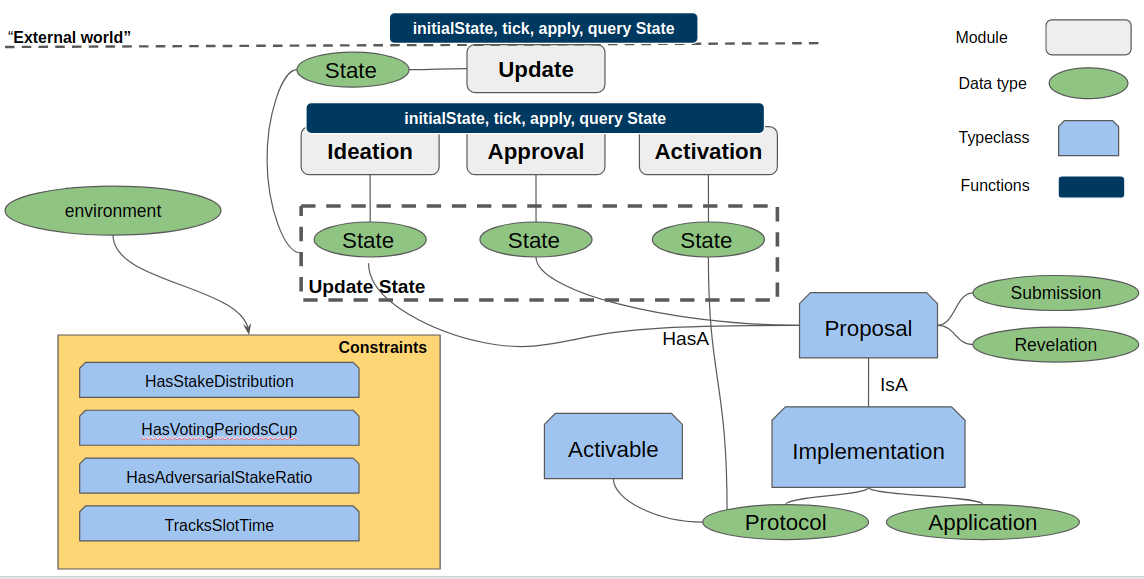
\includegraphics[width=0.8\columnwidth,
	keepaspectratio]{figures/update-system-sw-architecture.png}
	\caption{The update system software architecture.}
	\label{fig:upd-system-sw-architecture}
\end{figure}


Figure \ref{fig:upd-system-sw-architecture}, shows a very simplified view of 
the 
inner module structure of the update
system. The update module exposes a core set of functions (API) to the 
''external world'' that implement the ''update logic''. These are the 
\lstinline[language=Haskell]!initialState!, 
\lstinline[language=Haskell]!tick! and \lstinline[language=Haskell]!apply! 
functions discussed above and also a 
set of functions for querying the update state. Essentially each invocation of 
one of these three functions updates the internal (update) state. This state 
can be accessed via the query interface.

The update module dispatches the update payload to any of the 
ideation,
approval, and activation modules, depending on the payload type. These modules 
correspond to the respective phases in the lifecycle of a software update 
depicted in figure \ref{fig:su_lifecycle} and expose the same set of functions 
as the update module, specialized to the specific payload. 
The approval
module depends on the ideation module to provide information about which SIP's
have been approved and can proceed to the approval phase. The activation module
relies on the approval module to obtain information about which implementations
can proceed to the activation phase. All these module have their own private
state, which can be accessed only through their interfaces to it. The update
state includes these three states.

All states require that the data stored corresponds to instances of the
\lstinline[language=Haskell]!Proposal! typeclass. The 
\lstinline[language=Haskell]!Implementation! typeclass, depicted in the figure, 
is a further elaboration of the \lstinline[language=Haskell]!Proposal! 
typeclass specific to implementation proposals (a.k.a. UPs). As you can see, an 
implementation proposal needs to implement either a 
\lstinline[language=Haskell]!Protocol! change, or an 
\lstinline[language=Haskell]!Appplication! change. With the latter, we mean a 
software update that does not impact the consensus protocol. Moreover, as 
discussed above,
the protocol changes in particular, must be also instances of the 
\lstinline[language=Haskell]!Activable! typeclass. 
This enables certain attributes to the software update that have to do with the 
synchronization (endorsement period) prior to the activation of the change, 
which is imperative for protocol updates, in order to avoid chain splits.

Finally, all the exposed functions from the modules depicted, require an 
\emph{environment} input parameter. This can correspond to any environment data 
type, as long it honors a specific set of \emph{constraints}, expressed through 
a group of typeclasses, depicted in the figure. In particular,the ideation and 
approval 
\lstinline[language=Haskell]!State! modules
make use of the \lstinline[language=Haskell]!HasStakeDistribution!,
\lstinline[language=Haskell]!HasVotingPeriodsCap!, 
\lstinline[language=Haskell]!HasAdversarialStakeRatio!, and
\lstinline[language=Haskell]!TracksSlotTime! type classes for registering and 
tally votes. Since
the activation state only deals with endorsements, it only uses the assumption
that the environments passed to it tracks the slot time.
